\section{PoD共识算法}
\label{sec:PoD}

\subsection{常用共识算法的缺陷}
\label{PoD:weakness}

经典PoW (Proof of Work)共识算法为零和博弈,采用竞争性哈希计算来确定记账人,导致了整个生态每次出块时都有大量电能在竞争中被无端消耗,挖矿成本高。如果把公链参与者作为整体来看,PoW协议下生态维持平稳出块的成本将会持续升高。不断增加挖矿难度的Bitcoin早晚需要面临矿机收益入不敷出的情形,而Ethereum则早已在考虑使用新的PoS共识算法Casper~\cite{casper}来逐步取代现阶段的PoW共识~\cite{buterin2013ethereum}。

PoS (Proof of Stake)共识算法试图采用资产的多寡来取代算力的作用,按照币龄或者押金数额来分配获得记账权的概率,现阶段Peercoin~\cite{king2012peercoin}和Ethereum的Casper协议都采用了PoS共识算法。这种算法解决了PoW高能耗的弊端,但夸大了资本对记账权概率分配的影响,相较于PoW,在PoS下大资本更容易占据生态的话语权,形成大集团垄断,不利于公链生态的自由发展。

PoI (Proof of ImPoDtance)共识算法最早由Nem提出~\cite{nem},不同于PoS,PoI中引入了账户重要程度的概念,使用账户重要性评分来分配记账权的概率。这种算法解决了PoW的高能耗弊端,减缓了PoS的资本垄断危机,但确暴露了nothing-at-stake的问题,作弊者制造新区块的成本很低,公链受到51\%攻击的风险较高。

考虑到常用共识算法的缺陷,Nebulas提出了基于账户贡献度的PoD (Proof of Devotion)算法,从强调重要性的PoI共识算法出发,融合PoS中的经济惩罚,利用PoS强化了PoI的安全性,而PoI则反向遏制了PoS的垄断性,为生态自由发展助力。

\subsection{PoD算法设计}
\label{PoD:design}

\subsubsection{新区块产生}
\label{PoD:design:block}

PoD选取生态中有声望的账户来参与产生新区块 (block),采用Nebulas Rank算法,排名Top N的账户被视为有影响力声望高的账户,这些账户自愿缴纳一定数量的Nas作为押金后则有资格成为新区块的验证者 (validator),参与记账。

给定验证者集合 (validators set)之后,PoD算法通过伪随机数来决定验证者集合中谁是新的区块的提议者 (proposer),即所有高声望的账户拥有相同的概率获得新区块的提议权,防止概率倾斜衍生垄断。

\subsubsection{验证者集合}
\label{PoD:design:validators}

PoD为应对验证者集合的动态变化,首先将验证者集合按照朝代(dynasty)做划分,一个朝代内验证者集合不会发生变化,然后将每100个区块定义为一个Epoch,在同一个Epoch中朝代不会发生变化。因此朝代的变更只会发生在Epoch交接时,此时将会考察上一个Epoch的第一个区块,如果此区块到达了finality状态,那么当前Epoch进入下一个朝代D1,否则延续上一个朝代D0不变,如图\ref{fig:epoch}所示。

\begin{figure}[h]
\centering
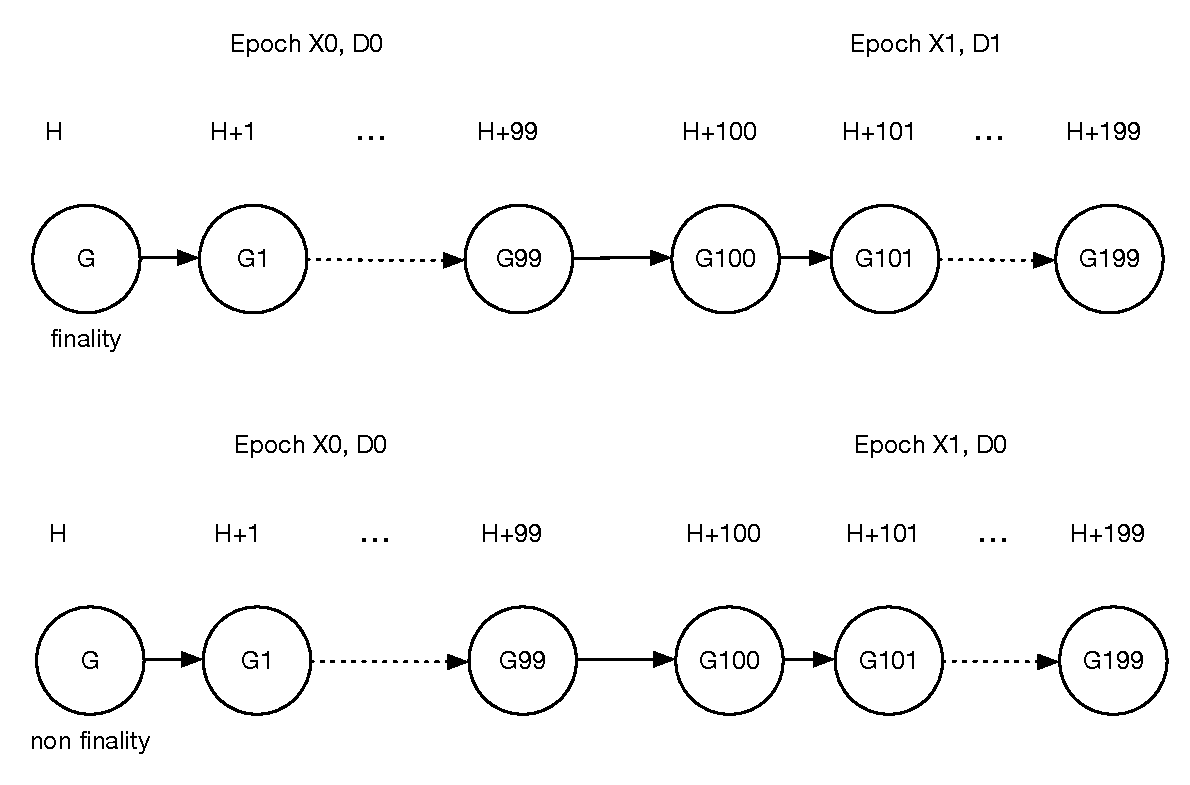
\includegraphics[width=8cm]{./figs/epoch}
\caption{验证者朝代更迭}
\label{fig:epoch}
\end{figure}

在任意一个朝代,有高声望的账户只能申请加入或者退出D+2朝代的验证者集合,当朝代变更到D+2时,即可加入新区块的共识过程,参与记账。

\subsubsection{共识过程}
\label{PoD:design:consensus}

新的区块被提出后,所有验证者将会参与一轮BFT (Byzantine Fault Tolerant)方式的投票,来确定此区块的合法性。在投票最开始,每一个参与此区块共识的验证者将会被收取$2x$ ($x$为激励奖金比例)的罚金,然后进入两阶段的投票过程。

\begin{itemize}
\item \textbf{第一阶段},所有验证者需要对新区块投$Prepare$票,投完$Prepare$票的验证者将获得$1.5x$的奖励,如果在当前朝代中有超过$2/3$的押金总额的验证者对新区块投了$Prepare$票,那么该区块进入投票的第二阶段。

\item \textbf{第二阶段},所有验证者需要对新区块投$Commit$票,投完$Commit$票的验证者,可以再获得1.5x的奖励,如果在当前朝代中有超过2/3的押金总额的验证者对新区块投了$Commit$票,那么该区块到达finality状态。
\end{itemize}

为了加速整个生态向前延展,对于任意在高度H的区块b,如果当前最新区块高度大于等于H+100,那么区块b将在共识过程中被视为过期,在过期的区块上产生的任何共识活动都将会被忽略。

\subsubsection{分叉选择}
\label{PoD:design:fork}

PoD算法以每个高度上区块的得分来选择权威链,总是选择得分最高的区块加入权威链,在高度h的区块b的得分如下,

\begin{align}
Score(b, h) = \sum_{(b',h') \in children(b)}Score(b', h') + \sum committed deposit in b
\end{align}
\noindent 即为该区块及其所有后代区块收到的commit票对应的押金总和,如图\ref{fig:fork_choice}所示。

\begin{figure}[h]
\centering
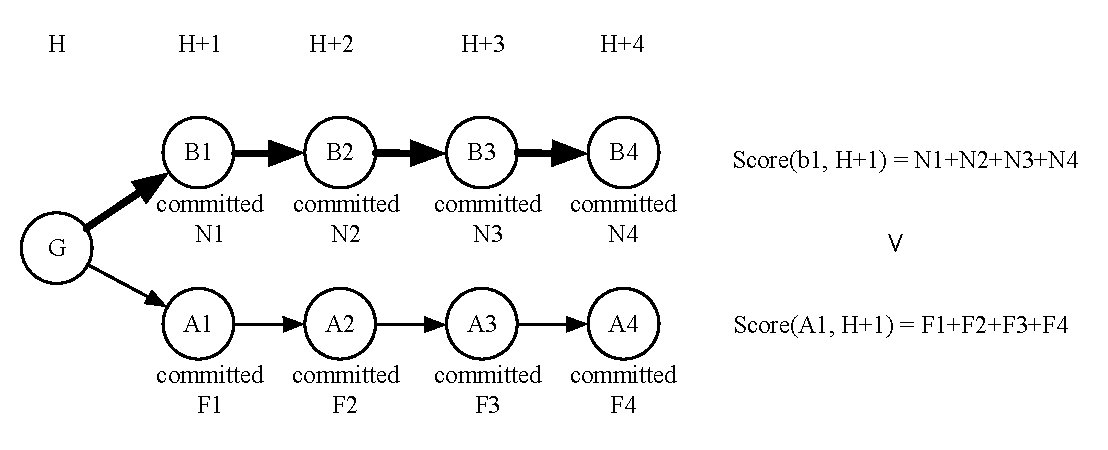
\includegraphics[width=12cm]{./figs/fork}
\caption{分叉选择}
\label{fig:fork_choice}
\end{figure}

\subsubsection{投票规则}
\label{PoD:design:vote}

为了避免共识过程被恶意破坏,导致共识过程没法完成,阻碍生态发展,PoD参考Casper的最小惩罚规则~\cite{minimal_slash_rules}来约束验证者的共识活动。

假设共识过程中的$Prepare$和$Commit$票结构如下,
\begin{itemize}
\item $Prepare(H, v, vs)$,其中$H$为当前区块hash,$v$表示当前区块高度,$vs$表示$v$的某个祖先区块高度
\item $Commit(H, v)$,其中H为当前区块hash,$v$表示当前区块高度
\end{itemize}

PoD算法为整个投票过程制定了如下4条基本规则,

\begin{itemize}
\item 单个区块的两阶段共识过程存在严格的先后顺序,只有在第一阶段$Prepare(H, v, vs)$票总权值达到$2/3$后,验证者们才可以投出第二阶段的$Commit(H, v)$票,
\item 多区块间不强制一个区块共识结束后才能开始后一个区块的共识,允许交织共识(interwoven consensus),但是不能完全没有秩序,只有高度vs完成了第一阶段过程,拥有$2/3$的$Prepare(H_anc, vs, vs’)$后,才可以基于vs对其后代区块投$Prepare(H, v, vs)$票,保证交织稳步向前
\item 为了避免有节点利用交织共识恶意跨多区块投票,要求基于高度u投出了$Prepare(H, w, u)$票之后,对于高度在跨度u和w之间的所有区块,不能再投出$Commit(H, v)$票,保证共识过程的高效有序
\item 为了制止节点用同一笔押金在多个分支上同时下注,导致Nothing at Stake的问题,要求在一个高度投出$Prepare(H1, v, vs1)$票之后,不能再投出不一样的$Prepare(H2, v, vs2)$票
\end{itemize}

违反上述规则的验证者一旦被举报核实,将会被罚掉所有押金,举报者们将会共享罚金的4\%作为奖励,罚金的剩余部分将会被销毁。

\subsection{PoD经济分析}
\label{PoD:economic}

\subsubsection{激励分析}
\label{PoD:economic:incentive}

参与PoD算法的验证者,在每一个合法区块上可以获得1x的星云币奖励,如果网络不畅或者有人作弊导致Prepare阶段没有办法完成进入Commit阶段,那么所有验证者将损失0.5x。因此成为验证者的价值节点在保持网络畅通,不参与作弊的情况下,将共享大量记账收益。

\subsubsection{作弊分析}
\label{PoD:economic:fraud}

\subsubsection*{双重支付攻击(double spend)}
\label{PoD:economic:fraud:double_spend}

假设商户merchant等到新区块到达finality状态就确认交易发货,那么fraud要在PoD共识算法下完成双重支付攻击实现零成本购物要付出的最小代价如下:

首先,fraud需要提高自己的Nebulas Rank到Top N,然后缴一定数的NaS作为押金成为验证者,并申请参与D+2朝代区块的验证。

然后,fraud需要被伪随机算法选中为新区块的提议者,此时fraud提出两个高度相同的新区块,一个哈希值为hash1包含fraud向merchant的转账交易,另一个哈希值为hash2包含fraud向fraud自己的转账交易。

最后,为了让hash1和hash2区块都到达finality,如图\ref{fig:double_spend}所示,fraud至少需要花费所有押金的$1/3$来贿赂$1/3$的验证者,让他们给两个区块都投$Commit$票。

\begin{figure}[h]
\centering
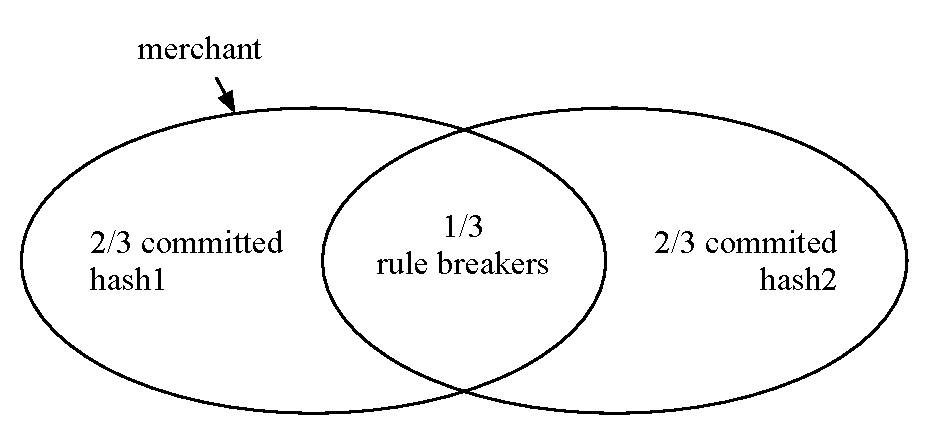
\includegraphics[width=7cm]{./figs/overlap}
\caption{双重支付经济惩罚}
\label{fig:double_spend}
\end{figure}

所以要完成一次成功的双重支付攻击,fraud需要花费一定的精力和财力来提升自己的Nebulas Rank排名(见 xxx Nebulas Rank排名经济分析),然后等到幸运地被选为提议者时,至少花费总押金的$1/3$来让两个块同时到达finality状态。

\subsubsection*{51\%攻击(51\% attack)}
\label{PoD:economic:fraud:51attack}

在PoW中要发起51\%攻击需要51\%的算力,在PoS中则需要51\%的押金,而在PoD中,则需要验证者集合中51\%的账户,这意味着拥有足够多的高声望用户进入Nebulas Rank的Top N,并且需要支付对应的押金,因此在PoD中51\%攻击将更为困难。

\subsubsection*{短程攻击(short-range attack)}
\label{PoD:economic:fraud:short_range_attack}

PoD中的每个高度上的区块都有共识有效期,如果某个高度距离最新高度超过100时,该高度的所有区块在共识过程中将被视为过期,那么这些区块上的所有新的共识活动将会被直接忽略。因此要在PoD中完成长程攻击(long-range attack)几乎不可能,但是在有效期内依旧存在发起短程攻击的可能性。

短程攻击者Attacker试图在高度H+1的区块还没有过期的情况下,伪造A链来替代B链成为权威链,Attacker需要让区块A1的得分比B1更高。由于多投会被严惩,所以Attacker将不可避免地要贿赂验证者,否则无法完成短程攻击。为了展现PoD共识算法的安全性,下面分别分析使不同数量的区块失效时,Attacker需要付出的代价。

如果Attacker想要使B1失效,最小代价的情况如图\ref{fig:revert1},就相当一次双重支付攻击,Attacker幸运地成为了H+1高度的区块提议者,那么至少需要贿赂朝代D0中$1/3$的验证者多投使A1达到finality,最小代价为所有押金的$1/3$。

\begin{figure}[h]
\centering
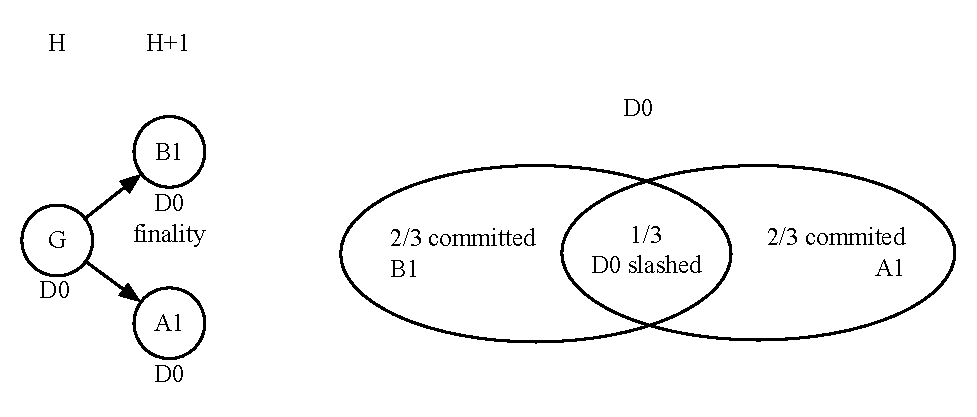
\includegraphics[width=11cm]{./figs/revert1}
\caption{短程攻击使一个区块失效的情形}
\label{fig:revert1}
\end{figure}

如果Attacker想要使B1-B2失效,假设B1和B2都已到达finality,块中交易都已生效,为了让这些交易失效,这里考虑两种情况。第一种如图\ref{fig:revert2}中(a)所示,高度H+1和H+2在同一个Epoch中,朝代相同,那么Attacker首先需要贿赂D0中$1/3$的验证者使A1达到finality,此时这$1/3$的验证者将会被惩罚,押金被罚完。在A2的验证中整体押金总和只有A1中的$2/3$,此时Attacker想要让A2到达和B2同价值的committ票,需要贿赂剩下所有没有作弊的验证者,合起来至少需要损失总押金的$3/3$,即使如此也不能保证A1得分比B1高,攻击失败风险高。第二种情况如图\ref{fig:revert2}中(b)所示,高度H+1和H+2正好在不同的Epoch中,且朝代不相同,那么此时Attacker需要贿赂D0中的$1/3$来让A1到达finality,然后贿赂D1中的$1/3$来让A2达到finality,完成一次这样的攻击至少需要损失总押金的$2/3$。综上,想要发起短程攻击导致两个finality区块失效,至少需要花费总押金$2/3$的代价。

\begin{figure}[h]
\centering
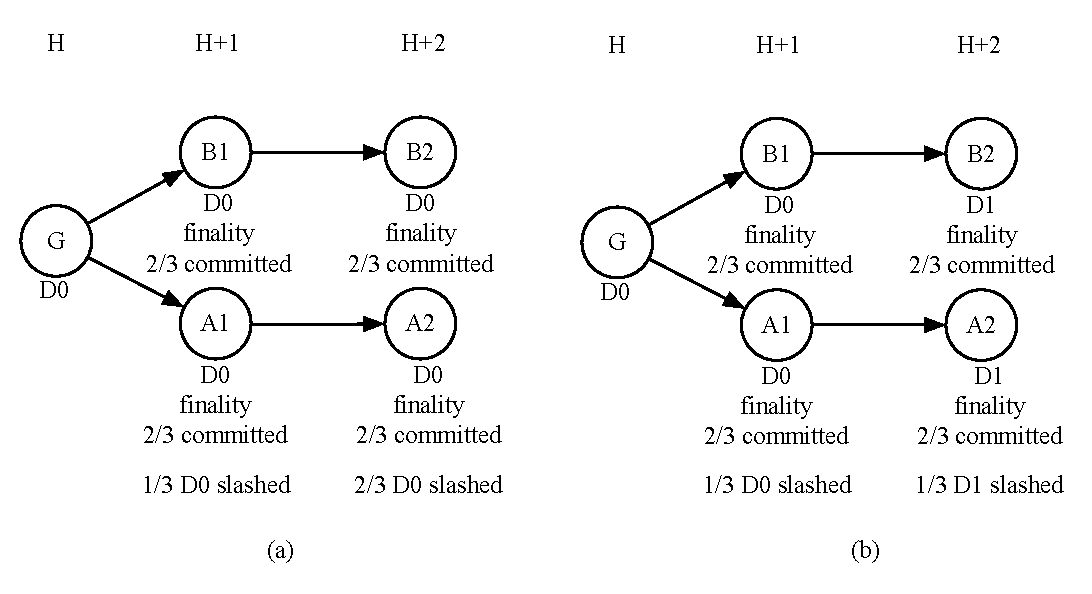
\includegraphics[width=11cm]{./figs/revert2}
\caption{短程攻击使两个区块失效的情形}
\label{fig:revert2}
\end{figure}


如果Attacker想要使B1-B3失效,如图\ref{fig:revert3}所示,Attacker首先需要贿赂D0中$1/3$的人完成A1的finality,然后贿赂D1中$1/3$的人完成A2的finality,最后需要贿赂D1中剩下$2/3$中的所有人来完成A3的finality,综上至少要损失总押金的$4/3$。要完成这些攻击准备将会十分困难,而且即使有幸做到了,也不定能保证A1的得分比B1高,攻击也可能会失败。

\begin{figure}[h]
\centering
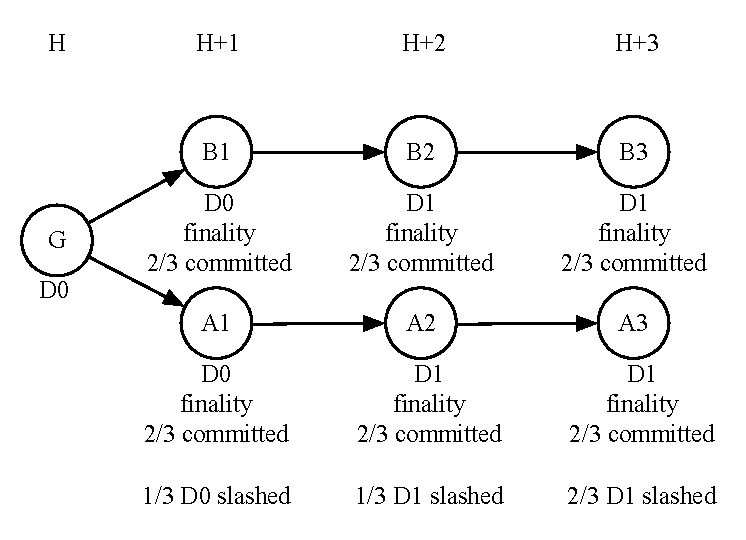
\includegraphics[width=7.5cm]{./figs/revert3}
\caption{短程攻击使三个区块失效的情形}
\label{fig:revert3}
\end{figure}

如果Attacker想要使B1-BN失效,其中N受到区块共识有效期的限制,不会很大,由于$N=3$时当前朝代所有验证者的押金就会被全部罚完,所以$N>=4$时,将没法完成攻击让B1得分比A1高,使B1\~BN失效,发起这样的攻击没有任何意义。
